% TODO: When to use bullets and when not?

\documentclass{article}

\usepackage{graphicx}
\usepackage{libertine}
\usepackage{libertinust1math}
\usepackage[T1]{fontenc}
%\usepackage{lmodern}
%\usepackage{fontspec}
%\setmainfont{Linux Libertine O}

\usepackage{xcolor}

\definecolor{tempborder}{rgb}{1, 1, 1} % hide temp borders
%\definecolor{tempborder}{rgb}{0.9, 0, 0.9} % show temp borders

\definecolor{strongblue}{rgb}{0.2, 0.3, 0.7} % main theme color

\usepackage{hyperref}
\hypersetup{
    colorlinks=true,
    linkcolor=strongblue,
    filecolor=strongblue,      
    urlcolor=strongblue,
}

\usepackage{pgfpages}
\usepackage{tikz}
\usetikzlibrary{calc}
\usetikzlibrary{matrix}
\usetikzlibrary{positioning}
\usepackage[active,tightpage]{preview}

%\usepackage{nicematrix}

\pgfdeclarelayer{background}
\pgfsetlayers{background,main}

\begin{document}
\begin{preview}

\def \mywebsite{https://mohnjahoney.github.io}



% Set independent lengths
\newcommand{\sidebarwidth}{6cm} % width of thin sidebar that runs down the side
\newcommand{\headerheight}{4cm} % height of header containing name and contact
\newcommand{\splitradius}{0.5cm} % split circle separates the four quadrants

\newcommand{\sectionpad}{0.4cm} % separation between section header and section and v.v.

\newcommand{\vennrad}{0.5*\headerheight}
\newcommand{\divisionlinewidth}{2pt}
\newcommand{\divisionlinepad}{0.5cm}
\newcommand{\bodytextinnersep}{4pt} %%%%%%%%%%%

% Compute dependent lengths
% TODO: can I really not do this with \newcommand??
% TODO: need to include line widths?
% TODO: I think inner sep in the text blocks is messing with things.
\pgfmathsetlengthmacro\bodywidth{\pdfpagewidth - \sidebarwidth - \divisionlinewidth}
\pgfmathsetlengthmacro\bodyheight{\pdfpageheight - \headerheight - \divisionlinewidth}
%\pgfmathsetlengthmacro\bodywidth{\pdfpagewidth - \sidebarwidth - 2*\splitradius}
%\pgfmathsetlengthmacro\bodyheight{\pdfpageheight - \headerheight - 2*\splitradius}

%%% TIKZPICTURE
\begin{tikzpicture} [
% Layout stuff
mat/.style={draw=tempborder, rectangle, matrix of nodes, rounded corners, line width=0.1pt, inner sep=0pt, outer sep=0pt, nodes={anchor=center}},
sec_title_mat/.style={mat, fill=white},%, text width=, text depth=}, % use matrix for organizing each section
sec_body_mat/.style={mat, fill=white},%, text width=, text depth=}, % use matrix for organizing each section
sidebar_body_mat/.style={mat, draw=tempborder, fill=strongblue!8!white},%, text width=, text depth=}, % use matrix for organizing each section
% Font stuff
sec_title/.style={font=\Large}, % section title
sec_title_circle/.style={draw=white, circle, line width=2pt, minimum width=0.4cm, anchor=center}, % circles used to demarkate section titles
sec_bold/.style={font=\bfseries\sffamily\normalsize, inner sep=\bodytextinnersep}, % bold "bullets" within each section
sec_text/.style={font=\sffamily\normalsize, inner sep=\bodytextinnersep}, % main text in each section
sidebar_text/.style={font=\sffamily\large, inner sep=\bodytextinnersep}, % main text in each section
%venn/.style={circle, draw=black!60, semithick, minimum size=5cm},
remember picture]

%% draw image
%\node[inner sep=0, opacity=0.3] at (current page)
%%{\includegraphics[width=\paperwidth,height=\paperheight]{poincare_mosaic.pdf}};
%{\includegraphics[width=\paperwidth,height=\paperheight]{me.png}};

%%% Split point - this is the main organizational coordinate
\node[draw=strongblue, circle, line width=2pt, minimum width=2*\splitradius, inner sep=0] (split) at (\sidebarwidth, \pdfpageheight - \headerheight) {};
%\coordinate(split) at (\sidebarwidth, \pdfpageheight - \headerheight);

\draw[strongblue, line width=\divisionlinewidth] (split.center) -- ++(\bodywidth, 0);
\draw[strongblue, line width=2pt] (split.center) -- ++(-\sidebarwidth, 0);
\draw[strongblue, line width=2pt] (split.center) -- ++(0, -\bodyheight);
\draw[strongblue, line width=2pt] (split.center) -- ++(0, \headerheight);

%%% Corner Icon
\begin{scope}
\clip ($(split.center) + (-\vennrad - \divisionlinewidth, \vennrad + \divisionlinewidth)$) circle (\vennrad);
\draw[draw=none, fill=yellow, opacity=1.0] (split.center) circle (1.0*\vennrad);
\end{scope}

%\draw[draw=black!20, line width=2pt] ($(split.center) + (-\vennrad - \divisionlinewidth, \vennrad + \divisionlinewidth)$) circle (\vennrad);
%\draw[draw=black!20, line width=2pt] ($(split.center) + (0, 0)$) +(45:\vennrad) arc (45:225:\vennrad);

% foliation
\begin{scope}
\clip ($(split.center) + (-\vennrad - \divisionlinewidth, \vennrad + \divisionlinewidth)$) circle (\vennrad);

% "normal" foliation
%\foreach \up in {3.1cm, 2.1cm, 1.2cm, 0.5cm, 0cm}{
%\filldraw[draw=black!50, semithick, fill=green, fill opacity=0.1] ($(split.center) + (-3*\vennrad, \up)$) -- ++(1.666*\vennrad + \up, 0cm) -- ++(\vennrad,-\vennrad) -- ++(0cm, -\vennrad) -- ++(-3*\vennrad, 0cm) -- cycle;

% fancy foliation
% start at center, move radially to edge, back up diagonally, then draw
%\foreach \up in {2.0cm, 1.6cm, 1.2cm, 0.8cm, 0.4cm, 0cm}{
%\foreach \up in {5, 4, 3, 2, 1, 0}{
%\filldraw[draw=black!50, line width=0.02*\up*1cm, fill=green, fill opacity=0.06] ($(split.center) + (-3*\vennrad, \up * 0.1cm)$) -- ++(1.666*\vennrad + 0.1*\up * 1cm, 0cm) -- ++(\vennrad,-\vennrad) -- ++(0cm, -\vennrad) -- ++(-3*\vennrad, 0cm) -- cycle;
\foreach \up in {7, 6, 5, 4, 3, 2, 1}{
\filldraw[draw=black!30, line width=1pt, fill=green, fill opacity=0.1] ($(split.center) + (-\vennrad, 0)$) -- (split.center) -- ++(\up*12+90:\vennrad) -- ++(-2*\vennrad, 0) -- ++(0, -2*\vennrad) -- cycle;
\draw[draw=black!20, line width=4pt] ($(split.center) + (-2*\vennrad, \vennrad)$) arc (180:0:\vennrad);
%\draw[] ($(split.center) + (-\vennrad, 0)$) arc 

% TODO: could use the control points to make foliation curved
%\filldraw[draw=black!60, semithick, fill=blue, fill opacity=0.1] ($(split.center) + (-\vennrad, \up)$) .. controls ++(-2,-2+\up) and (-1,0+\up) ..  (2,-1+\up) -- (3,0) -- (3,-5) -- (-3,-5) --   cycle;
}
\end{scope}


%%% Profile
\matrix[sec_body_mat, anchor=south west, line width=2pt, draw=none,
column 1/.style={sec_text, font=\large, text width=\bodywidth - \divisionlinepad}] (profile) at ($(split.center) + (\divisionlinepad, 1*\sectionpad)$) {
\emph{
I am a well-seasoned physicist, applied-math researcher, data scientist, and educator.
My experience spans time-series, information theory, reacting flows, and health informatics.
}\\
%\emph{
%I'm a rad dad who endeavors to make the world a fizzier place. 
%A physicist by training and jazz saxophonist by night, I approach the world with both an analytic mind and a the desire for a deep pocket.
%}\\
};

%\matrix[sec_title_mat, anchor=south west,
%row 1/.style={sec_title, anchor=center}] (profile_title) at ($(profile.north west) + (0.0cm, +\sectionpad)$) {
%\node[sec_title_circle, draw=black!20, fill=green, fill opacity=0.3 ] {};&
%~~PROFILE~~&
%\node[sec_title_circle] {};\\
%};


%%% NAME other design
\node[color=white, fill=strongblue, draw=none, line width=2pt, font=\huge, scale=1.8, rounded corners, anchor=south west] (name) at ($(profile.north west) + (0, 1*\sectionpad)$) {\textcolor{white}{~~~~John R. Mahoney~~~~}};


%%% Communication Skills
\matrix[sec_title_mat, anchor=north west,
row 1/.style={sec_title, anchor=center}] (communication_skills_title) at ($(split.center) + (\divisionlinepad, -2*\sectionpad)$) {
\node[sec_title_circle, draw=black!20, fill=green, fill opacity=0.5] {};&
~~COMMUNICATION~~&
\node[sec_title_circle] {};\\
};

\matrix[sec_body_mat, anchor=north west,
column 1/.style={sec_bold, text width=0.2*\bodywidth},
column 2/.style={sec_text, text width=0.8*\bodywidth - \divisionlinepad - 4*\bodytextinnersep}] (communication_skills) at ($(communication_skills_title.south west) + (0.0, -\sectionpad)$){
Written: &  Wrote and co-authored over 25 papers published in high-impact physics journals.
Lead to advancement of theory in: \href{https://mohnjahoney.github.io/pdfs/Times_Barbed_Arrow.pdf}{time-series prediction}, \href{https://mohnjahoney.github.io/pdfs/A_Turnstile_Mechanism_For_Fronts_Propagating_In_Fluid_Flows.pdf}{reacting fluid flows}, and \href{https://mohnjahoney.github.io/pdfs/Occams_Quantum_Strop.pdf}{quantum resource theory}; Important in securing co-authored grants from NSF (\$350k) and Templeton Foundation (\$440k).
%(PRL, PRX, PRA, PRE, CHAOS, J. Stat Phys.). 
% Edited multiple articles for colleagues.
%Refereed for several journals.
\\
%
Verbal: & Designed and delivered over 35 presentations 
%on time-series analysis, reacting fluid flows, and quantum information 
in venues such as Singapore, Amsterdam, Paris, Budapest, and Sendai.
%Quantum Info Workshop at Nanyang Technical University, Singapore;
%Conference on Complex Systems, Amsterdam;
%CHAOS15 at Henri Poincar\'e Institute, Paris;
%Oberwolfach, Germany
Awarded \href{https://mohnjahoney.github.io/pdfs/posters/Oberwolfach2014.pdf}{best poster} at ``Mixing, Transport, and Coherent Structures Workshop'' at the \href{https://www.mfo.de/}{MFO}.
Our theories have been applied in dozens of other theoretical and experimental works.
%International Conference on Flow Dynamics, Sendai, Japan
%International Conference on Nonlinear Science and Complexity, Budapest, Hungary
% TODO: add "Listen to: link to a talk I've given."
\\
Visual: & Value clarity, simplicity and aesthetics in communication. New \href{https://mohnjahoney.github.io/images/burning_front_topology.png}{reacting flow diagram} advances the canonical idea of phase portrait; applicable for heat transport and engine design. Promoted use of \href{https://mohnjahoney.github.io/images/FoliationCryptic.pdf}{Venn diagrams} for information theory; discovered new concepts of randomness and structure in time-series; impacted limits on algorithm design and computational architecture.
\\
%\href{https://mohnjahoney.github.io/images/quantum_strop_nemo.png}{quantum compression},
%\href{https://mohnjahoney.github.io/images/poincare_mosaic.pdf}{Poincar\'e art}\\
% TODO: add a video - maybe a BIM animation
%\phantom{blank} & Examples: \href{https://mohnjahoney.github.io/images/burning_front_topology.png}{A}, \href{https://mohnjahoney.github.io/images/quantum_strop_nemo.png}{B}, \href{https://mohnjahoney.github.io/images/poincare_mosaic.pdf}{C}\\
%\phantom{blank} & \node[draw=none] () {
%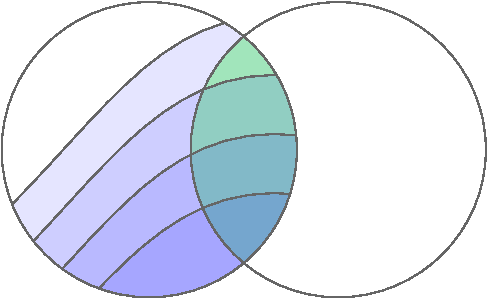
\includegraphics[width=2cm]{FoliationMarkov.pdf}
%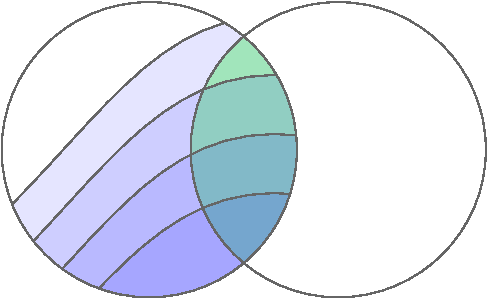
\includegraphics[width=2cm]{FoliationMarkov.pdf}};\\
};

%%% Analytical Skills
\matrix[sec_title_mat, anchor=north west,
row 1/.style={sec_title, anchor=center}] (analytical_skills_title) at ($(communication_skills.south west) + (0.0cm, -2*\sectionpad)$) {
\node[sec_title_circle, draw=black!20, fill=green, fill opacity=0.5] {};&
~~ANALYTICAL SKILLS~~&
\node[sec_title_circle] {};\\
};

\matrix[sec_body_mat, anchor=north west, 
column 1/.style={sec_bold, text width=0.2*\bodywidth},
column 2/.style={sec_text, text width=0.8*\bodywidth - \divisionlinepad - 4*\bodytextinnersep}] (analytical_skills) at ($(analytical_skills_title.south west) + (0.0cm, -\sectionpad)$) {
Research: & Connected my work on reacting fluids to existing fields: invariant manifolds, FT Lyapunov exponents, ARD equation, catastrophe theory, vehicle path planning, differential geometry.\\
Critical Thinking: & Reframed an assumption in the literature to build a fruitful research avenue - \textit{crypticity and cryptic order}. \\
Data and Code & Coding, simulation, statistical analysisCreated Python pipeline for data on diabetes patients: clean, process, analyze (multiple pair lagged regression), visualize. \\
};


%%% Work Experience
\matrix[sec_title_mat, anchor=north west,
row 1/.style={sec_title, anchor=center}] (work_experience_title) at ($(analytical_skills.south west) + (0.0cm, -2*\sectionpad)$) {
\node[sec_title_circle, draw=black!20, fill=green, fill opacity=0.5] {};&
~~WORK EXPERIENCE~~&
\node[sec_title_circle] {};\\
};

% TODO: There was some wrangling here to get the spacing right.
% Rows with letters that go below the baseline were making the spacing inconsistent.
% The style `nodes={anchor=center}` seems to have fixed that.
% text height=1.5ex, text depth=0.5ex
\matrix[sec_body_mat, anchor=north west, nodes={draw=none, line width=0.1pt},
column 1/.style={sec_bold, text width=0.2*\bodywidth},
column 2/.style={sec_text, text width=0.8*\bodywidth - \divisionlinepad - 4*\bodytextinnersep},
] (work_experience) at ($(work_experience_title.south west) + (0.0cm, -\sectionpad)$) {
Fall 2020&Math Specialist: UC Davis\\
Summer 2020&Course Designer and Instructor: UC Davis\\
Oct 2019&Math Lecturer: Napa Valley College\\
Spring 2019&Physics Lecturer: UC Davis\\
Fall 2018&Math Lecturer: CSU Maritime\\
2017-2018&Consultant: Dept. Biomedical Informatics, Columbia University\\
2017-2018&Math Lecturer: UC Davis\\
2015-2017&Project Scientist: UC Davis\\
2010-2015&Postdoctoral Scholar: UC Merced\\
};


%%% Education
\matrix[sec_title_mat, anchor=north west,
row 1/.style={sec_title, anchor=center}] (education_title) at ($(work_experience.south west) + (0.0cm, -2*\sectionpad)$) {
\node[sec_title_circle, draw=black!20, fill=green, fill opacity=0.5] {};&
~~EDUCATION~~&
\node[sec_title_circle] {};\\
};

\matrix[sec_body_mat, anchor=north west,
column 1/.style={sec_text, anchor=west}, text width=1.0*\bodywidth - \divisionlinepad - 2*\bodytextinnersep] (education) at ($(education_title.south west) + (0.0cm, -\sectionpad)$) {
Ph.D. in Physics, UC Davis, advisor: James P. Crutchfield\\
%�Extensions of the Theory of Computational Mechanics�
B.S. in Physics and Mathematics, CSU Chico\\
Williams College for Physics, Mathematics and Music\\
};


%%%%%%%%%%%
% Sidebar
%%%%%%%%%%%

%%% Interpersonal Skills
\matrix[sec_title_mat, anchor=north east,
row 1/.style={sec_title, anchor=center}] (interpersonal_skills_title) at ($(split.center) + (-\divisionlinepad, -2*\sectionpad)$) {
\node[sec_title_circle] {};&
~~INTERPERSONAL~~&
\node[sec_title_circle] {};\\
};

\matrix[sidebar_body_mat, anchor=north east, text width=1.0*\sidebarwidth  - \divisionlinepad - 2*\bodytextinnersep, align=right,
column 1/.style={sidebar_text}] (interpersonal_skills) at ($(interpersonal_skills_title.south east) + (0.0cm, -\sectionpad)$) {
Excellent listener\\
Flexible and creative\\
Work well in small teams\\
Independent worker\\
Thoughtful mentor\\%: (3 PhD, 7 undergrads)\\
};


%%% Coding Projects
\matrix[sec_title_mat, anchor=north east,
row 1/.style={sec_title, anchor=center}] (coding_projects_title) at ($(interpersonal_skills.south east) + (0.0cm, -2*\sectionpad)$) {
\node[sec_title_circle] {};&
~~CODING PROJECTS~~&
\node[sec_title_circle] {};\\
};

\matrix[sidebar_body_mat, anchor=north east, text width=1.0*\sidebarwidth - \divisionlinepad - 2*\bodytextinnersep, align=right,
column 1/.style={sidebar_text}] (coding_projects) at ($(coding_projects_title.south east) + (0.0cm, -\sectionpad)$) {
\href{https://github.com/mohnjahoney/magnacules}{Python \& Physics course}\\
\href{link}{Burning Invariant Manifolds}\\
\href{link}{CMPy} contributor\\
\href{https://github.com/mohnjahoney/simpsons_paradox}{Simpson's Paradox}\\
\href{link}{timesquare}\\
\href{https://github.com/mohnjahoney/resume}{r\'esum\'e template}\\
};


%%% Programming Skills
\matrix[sec_title_mat, anchor=north east,
row 1/.style={sec_title, anchor=center}] (programming_skills_title) at ($(coding_projects.south east) + (0.0cm, -2*\sectionpad)$) {
\node[sec_title_circle] {};&
~~PROGRAMMING~~&
\node[sec_title_circle] {};\\
};

%column 1/.style={font=\bfseries\Large, text width=0.2*\bodywidth},
%column 2/.style={text width=0.7*\bodywidth}
\matrix[sidebar_body_mat, anchor=north east, text width=1.0*\sidebarwidth - \divisionlinepad - 2*\bodytextinnersep, align=right, 
column 1/.style={sidebar_text, anchor=west}] (programming_skills) at ($(programming_skills_title.south east) + (0.0cm, -\sectionpad)$) {
Python: np, sp, mpl, pd\\
GUI / interactive\\
git, \LaTeX, beamer, tikz\\
ipython, Jupyter, VS Code\\
MATLAB\\
Mac OS, UNIX\\
};


%%% INTERESTS
\matrix[sec_title_mat, anchor=north east,
row 1/.style={sec_title, anchor=center}] (interests_title) at ($(programming_skills.south east) + (0.0cm, -2*\sectionpad)$) {
\node[sec_title_circle] {};&
~~INTERESTS~~&
\node[sec_title_circle] {};\\
};

\matrix[sidebar_body_mat, anchor=north east, text width=1.0*\sidebarwidth - \divisionlinepad - 2*\bodytextinnersep, align=right,
column 1/.style={sidebar_text}] (interests) at ($(interests_title.south east) + (0.0cm, -\sectionpad)$) {
Jazz saxophone and piano\\
Soccer, tennis, and hiking\\
Cooking delicious food!\\
};


\matrix[mat, anchor=north east, sidebar_text,
inner sep=\bodytextinnersep, draw=none, line width=2pt, fill=white, fill opacity=0.5, draw opacity=1.0, text opacity=1.0] (contact) at ($(interests.south east) + (0.0cm, -2*\sectionpad)$) {
mohnjahoney@gmail.com\\
(530) 601-0524\\
\href{\mywebsite}{mohnjahoney.github.io}\\
\node[draw=none, line width=3pt, rectangle] (gh) {
\href{https://github.com/mohnjahoney}{
\includegraphics[width=0.8cm]{github.pdf}}
\quad
\href{https://www.linkedin.com/in/johnmahoney3}{
\includegraphics[width=0.8cm]{LI-In-Bug.png}}
};\\
};


\end{tikzpicture}
\end{preview}
\end{document}
